\documentclass[10pt,compress,t,notes=noshow, xcolor=table]{beamer}

\usepackage[]{graphicx}
% graphicx is loaded via lmu-lecture.sty as well
\usepackage[]{color}
% maxwidth is the original width if it is less than linewidth
% otherwise use linewidth (to make sure the graphics do not exceed the margin)
\makeatletter
\def\maxwidth{ %
  \ifdim\Gin@nat@width>\linewidth
    \linewidth
  \else
    \Gin@nat@width
  \fi
}
\makeatother

% ---------------------------------%
% latex-math dependencies, do not remove:
% - mathtools
% - bm
% - siunitx
% - dsfont
% - xspace
% ---------------------------------%

%--------------------------------------------------------%
%       Language, encoding, typography
%--------------------------------------------------------%

\usepackage[english]{babel}
\usepackage[utf8]{inputenc} % Enables inputting UTF-8 symbols
% Standard AMS suite (loaded via lmu-lecture.sty)
\usepackage{amsmath,amsfonts,amssymb}

% Font for double-stroke / blackboard letters for sets of numbers (N, R, ...)
% Distribution name is "doublestroke"
% According to https://mirror.physik.tu-berlin.de/pub/CTAN/fonts/doublestroke/dsdoc.pdf
% the "bbm" package does a similar thing and may be superfluous.
% Required for latex-math
\usepackage{dsfont}

% bbm – "Blackboard-style" cm fonts (https://www.ctan.org/pkg/bbm)
% Used to be in common.tex, loaded directly after this file
% Maybe superfluous given dsfont is loaded
% TODO: Check if really unused?
% \usepackage{bbm}

% bm – Access bold symbols in maths mode - https://ctan.org/pkg/bm
% Required for latex-math, preferred over \boldsymbol
% https://tex.stackexchange.com/questions/3238/bm-package-versus-boldsymbol
\usepackage{bm}

% pifont – Access to PostScript standard Symbol and Dingbats fonts
% Used for \newcommand{\xmark}{\ding{55}, which is never used
% aside from lecture_advml/attic/xx-automl/slides.Rnw
% \usepackage{pifont}

% Quotes (inline and display), provdes \enquote
% https://ctan.org/pkg/csquotes
\usepackage{csquotes}

% Adds arg to enumerate env, technically superseded by enumitem according
% to https://ctan.org/pkg/enumerate
% Replace with https://ctan.org/pkg/enumitem ?
% Even better: enumitem is not really compatible with beamer and breaks all sorts of things
% particularly the enumerate environment. The enumerate package also just isn't required
% from what I can tell so... don't re-add it I guess?
% \usepackage{enumerate}

% Line spacing - provides \singlespacing \doublespacing \onehalfspacing
% https://ctan.org/pkg/setspace
% \usepackage{setspace}

% mathtools – Mathematical tools to use with amsmath
% https://ctan.org/pkg/mathtools?lang=en
% latex-math dependency according to latex-math repo
\usepackage{mathtools}

% Maybe not great to use this https://tex.stackexchange.com/a/197/19093
% Use align instead -- TODO: Global search & replace to check, eqnarray is used a lot
% $ rg -f -u "\begin{eqnarray" -l | grep -v attic | awk -F '/' '{print $1}' | sort | uniq -c
%   13 lecture_advml
%   14 lecture_i2ml
%    2 lecture_iml
%   27 lecture_optimization
%   45 lecture_sl
\usepackage{eqnarray}

% For shaded regions / boxes
% Used sometimes in optim
% https://www.ctan.org/pkg/framed
\usepackage{framed}

%--------------------------------------------------------%
%       Cite button (version 2024-05)
%--------------------------------------------------------%
% Note this requires biber to be in $PATH when running,
% telltale error in log would be e.g. Package biblatex Info: ... file 'authoryear.dbx' not found
% aside from obvious "biber: command not found" or similar.
% Tried moving this to lmu-lecture.sty but had issues I didn't quite understood,
% so it's here for now.

\usepackage{textcase} % for \NoCaseChange
\usepackage{hyperref}

% Only try adding a references file if it exists, otherwise
% this would compile error when references.bib is not found
\IfFileExists{references.bib} {
  \usepackage{usebib}
  \usepackage[backend=biber, style=authoryear]{biblatex}

  \addbibresource{./references.bib}
  \bibinput{references}
}

\newcommand{\citelink}[1]{%
\NoCaseChange{\resizebox{!}{9pt}{\protect\beamergotobutton{\href{\usebibentry{\NoCaseChange{#1}}{url}}{\begin{NoHyper}\cite{#1}\end{NoHyper}}}}}%
}

%--------------------------------------------------------%
%       Displaying code and algorithms
%--------------------------------------------------------%

% Reimplements verbatim environments: https://ctan.org/pkg/verbatim
% verbatim used sed at least once in
% supervised-classification/slides-classification-tasks.tex
% Removed since code should not be put on slides anyway
% \usepackage{verbatim}

% Both used together for algorithm typesetting, see also overleaf: https://www.overleaf.com/learn/latex/Algorithms
% algorithmic env is also used, but part of the bundle:
%   "algpseudocode is part of the algorithmicx bundle, it gives you an improved version of algorithmic besides providing some other features"
% According to https://tex.stackexchange.com/questions/229355/algorithm-algorithmic-algorithmicx-algorithm2e-algpseudocode-confused
\usepackage{algorithm}
\usepackage{algpseudocode}

%--------------------------------------------------------%
%       Tables
%--------------------------------------------------------%

% multi-row table cells: https://www.namsu.de/Extra/pakete/Multirow.html
% Provides \multirow
% Used e.g. in evaluation/slides-evaluation-measures-classification.tex
\usepackage{multirow}

% colortbl: https://ctan.org/pkg/colortbl
% "The package allows rows and columns to be coloured, and even individual cells." well.
% Provides \columncolor and \rowcolor
% \rowcolor is used multiple times, e.g. in knn/slides-knn.tex
\usepackage{colortbl}

% long/multi-page tables: https://texdoc.org/serve/longtable.pdf/0
% Not used in slides
% \usepackage{longtable}

% pretty table env: https://ctan.org/pkg/booktabs
% Is used
% Defines \toprule
\usepackage{booktabs}

%--------------------------------------------------------%
%       Figures: Creating, placing, verbing
%--------------------------------------------------------%

% wrapfig - Wrapping text around figures https://de.overleaf.com/learn/latex/Wrapping_text_around_figures
% Provides wrapfigure environment -used in lecture_optimization
\usepackage{wrapfig}

% Sub figures in figures and tables
% https://ctan.org/pkg/subfig -- supersedes subfigure package
% Provides \subfigure
% \subfigure not used in slides but slides-tuning-practical.pdf errors without this pkg, error due to \captionsetup undefined
\usepackage{subfig}

% Actually it's pronounced PGF https://en.wikibooks.org/wiki/LaTeX/PGF/TikZ
\usepackage{tikz}

% No idea what/why these settings are what they are but I assume they're there on purpose
\usetikzlibrary{shapes,arrows,automata,positioning,calc,chains,trees, shadows}
\tikzset{
  %Define standard arrow tip
  >=stealth',
  %Define style for boxes
  punkt/.style={
    rectangle,
    rounded corners,
    draw=black, very thick,
    text width=6.5em,
    minimum height=2em,
    text centered},
  % Define arrow style
  pil/.style={
    ->,
    thick,
    shorten <=2pt,
    shorten >=2pt,}
}

%--------------------------------------------------------%
%       Beamer setup and custom macros & environments
%--------------------------------------------------------%

% Main sty file for beamer setup (layout, style, lecture page numbering, etc.)
% For long-term maintenance, this may me refactored into a more modular set of .sty files
\usepackage{../../style/lmu-lecture}
% Custom itemize wrappers, itemizeS, itemizeL, etc
\usepackage{../../style/customitemize}
% Custom framei environment, uses custom itemize!
\usepackage{../../style/framei}
% Custom frame2 environment, allows specifying font size for all content
\usepackage{../../style/frame2}
% Column layout macros
\usepackage{../../style/splitV} 

% Used regularly
\let\code=\texttt

% Not sure what/why this does
\setkeys{Gin}{width=0.9\textwidth}

% -- knitr leftovers --
% Used often in conjunction with \definecolor{shadecolor}{rgb}{0.969, 0.969, 0.969}
% Removing definitions requires chaning _many many_ slides, which then need checking to see if output still ok
\definecolor{fgcolor}{rgb}{0.345, 0.345, 0.345}
\definecolor{shadecolor}{rgb}{0.969, 0.969, 0.969}
\newenvironment{knitrout}{}{} % an empty environment to be redefined in TeX

%-------------------------------------------------------------------------------------------------------%
%  Unused stuff that needs to go but is kept here currently juuuust in case it was important after all  %
%-------------------------------------------------------------------------------------------------------%

% \newcommand{\hlnum}[1]{\textcolor[rgb]{0.686,0.059,0.569}{#1}}%
% \newcommand{\hlstr}[1]{\textcolor[rgb]{0.192,0.494,0.8}{#1}}%
% \newcommand{\hlcom}[1]{\textcolor[rgb]{0.678,0.584,0.686}{\textit{#1}}}%
% \newcommand{\hlopt}[1]{\textcolor[rgb]{0,0,0}{#1}}%
% \newcommand{\hlstd}[1]{\textcolor[rgb]{0.345,0.345,0.345}{#1}}%
% \newcommand{\hlkwa}[1]{\textcolor[rgb]{0.161,0.373,0.58}{\textbf{#1}}}%
% \newcommand{\hlkwb}[1]{\textcolor[rgb]{0.69,0.353,0.396}{#1}}%
% \newcommand{\hlkwc}[1]{\textcolor[rgb]{0.333,0.667,0.333}{#1}}%
% \newcommand{\hlkwd}[1]{\textcolor[rgb]{0.737,0.353,0.396}{\textbf{#1}}}%
% \let\hlipl\hlkwb

% \makeatletter
% \newenvironment{kframe}{%
%  \def\at@end@of@kframe{}%
%  \ifinner\ifhmode%
%   \def\at@end@of@kframe{\end{minipage}}%
%   \begin{minipage}{\columnwidth}%
%  \fi\fi%
%  \def\FrameCommand##1{\hskip\@totalleftmargin \hskip-\fboxsep
%  \colorbox{shadecolor}{##1}\hskip-\fboxsep
%      % There is no \\@totalrightmargin, so:
%      \hskip-\linewidth \hskip-\@totalleftmargin \hskip\columnwidth}%
%  \MakeFramed {\advance\hsize-\width
%    \@totalleftmargin\z@ \linewidth\hsize
%    \@setminipage}}%
%  {\par\unskip\endMakeFramed%
%  \at@end@of@kframe}
% \makeatother

% \definecolor{shadecolor}{rgb}{.97, .97, .97}
% \definecolor{messagecolor}{rgb}{0, 0, 0}
% \definecolor{warningcolor}{rgb}{1, 0, 1}
% \definecolor{errorcolor}{rgb}{1, 0, 0}
% \newenvironment{knitrout}{}{} % an empty environment to be redefined in TeX

% \usepackage{alltt}
% \newcommand{\SweaveOpts}[1]{}  % do not interfere with LaTeX
% \newcommand{\SweaveInput}[1]{} % because they are not real TeX commands
% \newcommand{\Sexpr}[1]{}       % will only be parsed by R
% \newcommand{\xmark}{\ding{55}}%

% textpos – Place boxes at arbitrary positions on the LATEX page
% https://ctan.org/pkg/textpos
% Provides \begin{textblock}
% TODO: Check if really unused?
% \usepackage[absolute,overlay]{textpos}

% -----------------------%
% Likely knitr leftovers %
% -----------------------%

% psfrag – Replace strings in encapsulated PostScript figures
% https://www.overleaf.com/latex/examples/psfrag-example/tggxhgzwrzhn
% https://ftp.mpi-inf.mpg.de/pub/tex/mirror/ftp.dante.de/pub/tex/macros/latex/contrib/psfrag/pfgguide.pdf
% Can't tell if this is needed
% TODO: Check if really unused?
% \usepackage{psfrag}

% arydshln – Draw dash-lines in array/tabular
% https://www.ctan.org/pkg/arydshln
% !! "arydshln has to be loaded after array, longtable, colortab and/or colortbl"
% Provides \hdashline and \cdashline
% Not used in slides
% \usepackage{arydshln}

% tabularx – Tabulars with adjustable-width columns
% https://ctan.org/pkg/tabularx
% Provides \begin{tabularx}
% Not used in slides
% \usepackage{tabularx}

% placeins – Control float placement
% https://ctan.org/pkg/placeins
% Defines a \FloatBarrier command
% TODO: Check if really unused?
% \usepackage{placeins}

% Can't find a reason why common.tex is not just part of this file?
% This file is included in slides and exercises

% Rarely used fontstyle for R packages, used only in 
% - forests/slides-forests-benchmark.tex
% - exercises/single-exercises/methods_l_1.Rnw
% - slides/cart/attic/slides_extra_trees.Rnw
\newcommand{\pkg}[1]{{\fontseries{b}\selectfont #1}}

% Spacing helpers, used often (mostly in exercises for \dlz)
\newcommand{\lz}{\vspace{0.5cm}} % vertical space (used often in slides)
\newcommand{\dlz}{\vspace{1cm}}  % double vertical space (used often in exercises, never in slides)
\newcommand{\oneliner}[1] % Oneliner for important statements, used e.g. in iml, algods
{\begin{block}{}\begin{center}\begin{Large}#1\end{Large}\end{center}\end{block}}

% Don't know if this is used or needed, remove?
% textcolor that works in mathmode
% https://tex.stackexchange.com/a/261480
% Used e.g. in forests/slides-forests-bagging.tex
% [...] \textcolor{blue}{\tfrac{1}{M}\sum^M_{m} [...]
% \makeatletter
% \renewcommand*{\@textcolor}[3]{%
%   \protect\leavevmode
%   \begingroup
%     \color#1{#2}#3%
%   \endgroup
% }
% \makeatother


% dependencies: amsmath, amssymb, dsfont
% math spaces
\ifdefined\N
\renewcommand{\N}{\mathds{N}} % N, naturals
\else \newcommand{\N}{\mathds{N}} \fi
\newcommand{\Z}{\mathds{Z}} % Z, integers
\newcommand{\Q}{\mathds{Q}} % Q, rationals
\newcommand{\R}{\mathds{R}} % R, reals
\ifdefined\C
\renewcommand{\C}{\mathds{C}} % C, complex
\else \newcommand{\C}{\mathds{C}} \fi
\newcommand{\continuous}{\mathcal{C}} % C, space of continuous functions
\newcommand{\M}{\mathcal{M}} % machine numbers
\newcommand{\epsm}{\epsilon_m} % maximum error

% counting / finite sets
\newcommand{\setzo}{\{0, 1\}} % set 0, 1
\newcommand{\setmp}{\{-1, +1\}} % set -1, 1
\newcommand{\unitint}{[0, 1]} % unit interval

% basic math stuff
\newcommand{\xt}{\tilde x} % x tilde
\DeclareMathOperator*{\argmax}{arg\,max} % argmax
\DeclareMathOperator*{\argmin}{arg\,min} % argmin
\newcommand{\argminlim}{\mathop{\mathrm{arg\,min}}\limits} % argmax with limits
\newcommand{\argmaxlim}{\mathop{\mathrm{arg\,max}}\limits} % argmin with limits
\newcommand{\sign}{\operatorname{sign}} % sign, signum
\newcommand{\I}{\mathbb{I}} % I, indicator
\newcommand{\order}{\mathcal{O}} % O, order
\newcommand{\bigO}{\mathcal{O}} % Big-O Landau
\newcommand{\littleo}{{o}} % Little-o Landau
\newcommand{\pd}[2]{\frac{\partial{#1}}{\partial #2}} % partial derivative
\newcommand{\floorlr}[1]{\left\lfloor #1 \right\rfloor} % floor
\newcommand{\ceillr}[1]{\left\lceil #1 \right\rceil} % ceiling
\newcommand{\indep}{\perp \!\!\! \perp} % independence symbol

% sums and products
\newcommand{\sumin}{\sum\limits_{i=1}^n} % summation from i=1 to n
\newcommand{\sumim}{\sum\limits_{i=1}^m} % summation from i=1 to m
\newcommand{\sumjn}{\sum\limits_{j=1}^n} % summation from j=1 to p
\newcommand{\sumjp}{\sum\limits_{j=1}^p} % summation from j=1 to p
\newcommand{\sumik}{\sum\limits_{i=1}^k} % summation from i=1 to k
\newcommand{\sumkg}{\sum\limits_{k=1}^g} % summation from k=1 to g
\newcommand{\sumjg}{\sum\limits_{j=1}^g} % summation from j=1 to g
\newcommand{\summM}{\sum\limits_{m=1}^M} % summation from m=1 to M
\newcommand{\meanin}{\frac{1}{n} \sum\limits_{i=1}^n} % mean from i=1 to n
\newcommand{\meanim}{\frac{1}{m} \sum\limits_{i=1}^m} % mean from i=1 to n
\newcommand{\meankg}{\frac{1}{g} \sum\limits_{k=1}^g} % mean from k=1 to g
\newcommand{\meanmM}{\frac{1}{M} \sum\limits_{m=1}^M} % mean from m=1 to M
\newcommand{\prodin}{\prod\limits_{i=1}^n} % product from i=1 to n
\newcommand{\prodkg}{\prod\limits_{k=1}^g} % product from k=1 to g
\newcommand{\prodjp}{\prod\limits_{j=1}^p} % product from j=1 to p

% linear algebra
\newcommand{\one}{\bm{1}} % 1, unitvector
\newcommand{\zero}{\mathbf{0}} % 0-vector
\newcommand{\id}{\bm{I}} % I, identity
\newcommand{\diag}{\operatorname{diag}} % diag, diagonal
\newcommand{\trace}{\operatorname{tr}} % tr, trace
\newcommand{\spn}{\operatorname{span}} % span
\newcommand{\scp}[2]{\left\langle #1, #2 \right\rangle} % <.,.>, scalarproduct
\newcommand{\mat}[1]{\begin{pmatrix} #1 \end{pmatrix}} % short pmatrix command
\newcommand{\Amat}{\mathbf{A}} % matrix A
\newcommand{\Deltab}{\mathbf{\Delta}} % error term for vectors

% basic probability + stats
\renewcommand{\P}{\mathds{P}} % P, probability
\newcommand{\E}{\mathds{E}} % E, expectation
\newcommand{\var}{\mathsf{Var}} % Var, variance
\newcommand{\cov}{\mathsf{Cov}} % Cov, covariance
\newcommand{\corr}{\mathsf{Corr}} % Corr, correlation
\newcommand{\normal}{\mathcal{N}} % N of the normal distribution
\newcommand{\iid}{\overset{i.i.d}{\sim}} % dist with i.i.d superscript
\newcommand{\distas}[1]{\overset{#1}{\sim}} % ... is distributed as ...

% machine learning
\newcommand{\Xspace}{\mathcal{X}} % X, input space
\newcommand{\Yspace}{\mathcal{Y}} % Y, output space
\newcommand{\Zspace}{\mathcal{Z}} % Z, space of sampled datapoints
\newcommand{\nset}{\{1, \ldots, n\}} % set from 1 to n
\newcommand{\pset}{\{1, \ldots, p\}} % set from 1 to p
\newcommand{\gset}{\{1, \ldots, g\}} % set from 1 to g
\newcommand{\Pxy}{\mathbb{P}_{xy}} % P_xy
\newcommand{\Exy}{\mathbb{E}_{xy}} % E_xy: Expectation over random variables xy
\newcommand{\xv}{\mathbf{x}} % vector x (bold)
\newcommand{\xtil}{\tilde{\mathbf{x}}} % vector x-tilde (bold)
\newcommand{\yv}{\mathbf{y}} % vector y (bold)
\newcommand{\xy}{(\xv, y)} % observation (x, y)
\newcommand{\xvec}{\left(x_1, \ldots, x_p\right)^\top} % (x1, ..., xp)
\newcommand{\Xmat}{\mathbf{X}} % Design matrix
\newcommand{\allDatasets}{\mathds{D}} % The set of all datasets
\newcommand{\allDatasetsn}{\mathds{D}_n}  % The set of all datasets of size n
\newcommand{\D}{\mathcal{D}} % D, data
\newcommand{\Dn}{\D_n} % D_n, data of size n
\newcommand{\Dtrain}{\mathcal{D}_{\text{train}}} % D_train, training set
\newcommand{\Dtest}{\mathcal{D}_{\text{test}}} % D_test, test set
\newcommand{\xyi}[1][i]{\left(\xv^{(#1)}, y^{(#1)}\right)} % (x^i, y^i), i-th observation
\newcommand{\Dset}{\left( \xyi[1], \ldots, \xyi[n]\right)} % {(x1,y1)), ..., (xn,yn)}, data
\newcommand{\defAllDatasetsn}{(\Xspace \times \Yspace)^n} % Def. of the set of all datasets of size n
\newcommand{\defAllDatasets}{\bigcup_{n \in \N}(\Xspace \times \Yspace)^n} % Def. of the set of all datasets
\newcommand{\xdat}{\left\{ \xv^{(1)}, \ldots, \xv^{(n)}\right\}} % {x1, ..., xn}, input data
\newcommand{\ydat}{\left\{ \yv^{(1)}, \ldots, \yv^{(n)}\right\}} % {y1, ..., yn}, input data
\newcommand{\yvec}{\left(y^{(1)}, \hdots, y^{(n)}\right)^\top} % (y1, ..., yn), vector of outcomes
\newcommand{\greekxi}{\xi} % Greek letter xi
\renewcommand{\xi}[1][i]{\xv^{(#1)}} % x^i, i-th observed value of x
\newcommand{\yi}[1][i]{y^{(#1)}} % y^i, i-th observed value of y
\newcommand{\xivec}{\left(x^{(i)}_1, \ldots, x^{(i)}_p\right)^\top} % (x1^i, ..., xp^i), i-th observation vector
\newcommand{\xj}{\xv_j} % x_j, j-th feature
\newcommand{\xjvec}{\left(x^{(1)}_j, \ldots, x^{(n)}_j\right)^\top} % (x^1_j, ..., x^n_j), j-th feature vector
\newcommand{\phiv}{\mathbf{\phi}} % Basis transformation function phi
\newcommand{\phixi}{\mathbf{\phi}^{(i)}} % Basis transformation of xi: phi^i := phi(xi)

%%%%%% ml - models general
\newcommand{\lamv}{\bm{\lambda}} % lambda vector, hyperconfiguration vector
\newcommand{\Lam}{\bm{\Lambda}}	 % Lambda, space of all hpos
% Inducer / Inducing algorithm
\newcommand{\preimageInducer}{\left(\defAllDatasets\right)\times\Lam} % Set of all datasets times the hyperparameter space
\newcommand{\preimageInducerShort}{\allDatasets\times\Lam} % Set of all datasets times the hyperparameter space
% Inducer / Inducing algorithm
\newcommand{\ind}{\mathcal{I}} % Inducer, inducing algorithm, learning algorithm

% continuous prediction function f
\newcommand{\ftrue}{f_{\text{true}}}  % True underlying function (if a statistical model is assumed)
\newcommand{\ftruex}{\ftrue(\xv)} % True underlying function (if a statistical model is assumed)
\newcommand{\fx}{f(\xv)} % f(x), continuous prediction function
\newcommand{\fdomains}{f: \Xspace \rightarrow \R^g} % f with domain and co-domain
\newcommand{\Hspace}{\mathcal{H}} % hypothesis space where f is from
\newcommand{\fbayes}{f^{\ast}} % Bayes-optimal model
\newcommand{\fxbayes}{f^{\ast}(\xv)} % Bayes-optimal model
\newcommand{\fkx}[1][k]{f_{#1}(\xv)} % f_j(x), discriminant component function
\newcommand{\fh}{\hat{f}} % f hat, estimated prediction function
\newcommand{\fxh}{\fh(\xv)} % fhat(x)
\newcommand{\fxt}{f(\xv ~|~ \thetav)} % f(x | theta)
\newcommand{\fxi}{f\left(\xv^{(i)}\right)} % f(x^(i))
\newcommand{\fxih}{\hat{f}\left(\xv^{(i)}\right)} % f(x^(i))
\newcommand{\fxit}{f\left(\xv^{(i)} ~|~ \thetav\right)} % f(x^(i) | theta)
\newcommand{\fhD}{\fh_{\D}} % fhat_D, estimate of f based on D
\newcommand{\fhDtrain}{\fh_{\Dtrain}} % fhat_Dtrain, estimate of f based on D
\newcommand{\fhDnlam}{\fh_{\Dn, \lamv}} %model learned on Dn with hp lambda
\newcommand{\fhDlam}{\fh_{\D, \lamv}} %model learned on D with hp lambda
\newcommand{\fhDnlams}{\fh_{\Dn, \lamv^\ast}} %model learned on Dn with optimal hp lambda
\newcommand{\fhDlams}{\fh_{\D, \lamv^\ast}} %model learned on D with optimal hp lambda

% discrete prediction function h
\newcommand{\hx}{h(\xv)} % h(x), discrete prediction function
\newcommand{\hh}{\hat{h}} % h hat
\newcommand{\hxh}{\hat{h}(\xv)} % hhat(x)
\newcommand{\hxt}{h(\xv | \thetav)} % h(x | theta)
\newcommand{\hxi}{h\left(\xi\right)} % h(x^(i))
\newcommand{\hxit}{h\left(\xi ~|~ \thetav\right)} % h(x^(i) | theta)
\newcommand{\hbayes}{h^{\ast}} % Bayes-optimal classification model
\newcommand{\hxbayes}{h^{\ast}(\xv)} % Bayes-optimal classification model

% yhat
\newcommand{\yh}{\hat{y}} % yhat for prediction of target
\newcommand{\yih}{\hat{y}^{(i)}} % yhat^(i) for prediction of ith targiet
\newcommand{\resi}{\yi- \yih}

% theta
\newcommand{\thetah}{\hat{\theta}} % theta hat
\newcommand{\thetav}{\bm{\theta}} % theta vector
\newcommand{\thetavh}{\bm{\hat\theta}} % theta vector hat
\newcommand{\thetat}[1][t]{\thetav^{[#1]}} % theta^[t] in optimization
\newcommand{\thetatn}[1][t]{\thetav^{[#1 +1]}} % theta^[t+1] in optimization
\newcommand{\thetahDnlam}{\thetavh_{\Dn, \lamv}} %theta learned on Dn with hp lambda
\newcommand{\thetahDlam}{\thetavh_{\D, \lamv}} %theta learned on D with hp lambda
\newcommand{\mint}{\min_{\thetav \in \Theta}} % min problem theta
\newcommand{\argmint}{\argmin_{\thetav \in \Theta}} % argmin theta

% densities + probabilities
% pdf of x
\newcommand{\pdf}{p} % p
\newcommand{\pdfx}{p(\xv)} % p(x)
\newcommand{\pixt}{\pi(\xv~|~ \thetav)} % pi(x|theta), pdf of x given theta
\newcommand{\pixit}[1][i]{\pi\left(\xi[#1] ~|~ \thetav\right)} % pi(x^i|theta), pdf of x given theta
\newcommand{\pixii}[1][i]{\pi\left(\xi[#1]\right)} % pi(x^i), pdf of i-th x

% pdf of (x, y)
\newcommand{\pdfxy}{p(\xv,y)} % p(x, y)
\newcommand{\pdfxyt}{p(\xv, y ~|~ \thetav)} % p(x, y | theta)
\newcommand{\pdfxyit}{p\left(\xi, \yi ~|~ \thetav\right)} % p(x^(i), y^(i) | theta)

% pdf of x given y
\newcommand{\pdfxyk}[1][k]{p(\xv | y= #1)} % p(x | y = k)
\newcommand{\lpdfxyk}[1][k]{\log p(\xv | y= #1)} % log p(x | y = k)
\newcommand{\pdfxiyk}[1][k]{p\left(\xi | y= #1 \right)} % p(x^i | y = k)

% prior probabilities
\newcommand{\pik}[1][k]{\pi_{#1}} % pi_k, prior
\newcommand{\pih}{\hat{\pi}} % pi hat, estimated prior (binary classification)
\newcommand{\pikh}[1][k]{\hat{\pi}_{#1}} % pi_k hat, estimated prior
\newcommand{\lpik}[1][k]{\log \pi_{#1}} % log pi_k, log of the prior
\newcommand{\pit}{\pi(\thetav)} % Prior probability of parameter theta

% posterior probabilities
\newcommand{\post}{\P(y = 1 ~|~ \xv)} % P(y = 1 | x), post. prob for y=1
\newcommand{\postk}[1][k]{\P(y = #1 ~|~ \xv)} % P(y = k | y), post. prob for y=k
\newcommand{\pidomains}{\pi: \Xspace \rightarrow \unitint} % pi with domain and co-domain
\newcommand{\pibayes}{\pi^{\ast}} % Bayes-optimal classification model
\newcommand{\pixbayes}{\pi^{\ast}(\xv)} % Bayes-optimal classification model
\newcommand{\pix}{\pi(\xv)} % pi(x), P(y = 1 | x)
\newcommand{\piv}{\bm{\pi}} % pi, bold, as vector
\newcommand{\pikx}[1][k]{\pi_{#1}(\xv)} % pi_k(x), P(y = k | x)
\newcommand{\pikxt}[1][k]{\pi_{#1}(\xv ~|~ \thetav)} % pi_k(x | theta), P(y = k | x, theta)
\newcommand{\pixh}{\hat \pi(\xv)} % pi(x) hat, P(y = 1 | x) hat
\newcommand{\pikxh}[1][k]{\hat \pi_{#1}(\xv)} % pi_k(x) hat, P(y = k | x) hat
\newcommand{\pixih}{\hat \pi(\xi)} % pi(x^(i)) with hat
\newcommand{\pikxih}[1][k]{\hat \pi_{#1}(\xi)} % pi_k(x^(i)) with hat
\newcommand{\pdfygxt}{p(y ~|~\xv, \thetav)} % p(y | x, theta)
\newcommand{\pdfyigxit}{p\left(\yi ~|~\xi, \thetav\right)} % p(y^i |x^i, theta)
\newcommand{\lpdfygxt}{\log \pdfygxt } % log p(y | x, theta)
\newcommand{\lpdfyigxit}{\log \pdfyigxit} % log p(y^i |x^i, theta)

% probababilistic
\newcommand{\bayesrulek}[1][k]{\frac{\P(\xv | y= #1) \P(y= #1)}{\P(\xv)}} % Bayes rule
\newcommand{\muv}{\bm{\mu}} % expectation vector of Gaussian
\newcommand{\muk}[1][k]{\bm{\mu_{#1}}} % mean vector of class-k Gaussian (discr analysis)
\newcommand{\mukh}[1][k]{\bm{\hat{\mu}_{#1}}} % estimated mean vector of class-k Gaussian (discr analysis)

% residual and margin
\newcommand{\eps}{\epsilon} % residual, stochastic
\newcommand{\epsv}{\bm{\epsilon}} % residual, stochastic, as vector
\newcommand{\epsi}{\epsilon^{(i)}} % epsilon^i, residual, stochastic
\newcommand{\epsh}{\hat{\epsilon}} % residual, estimated
\newcommand{\epsvh}{\hat{\epsv}} % residual, estimated, vector
\newcommand{\yf}{y \fx} % y f(x), margin
\newcommand{\yfi}{\yi \fxi} % y^i f(x^i), margin
\newcommand{\Sigmah}{\hat \Sigma} % estimated covariance matrix
\newcommand{\Sigmahj}{\hat \Sigma_j} % estimated covariance matrix for the j-th class

% ml - loss, risk, likelihood
\newcommand{\Lyf}{L\left(y, f\right)} % L(y, f), loss function
\newcommand{\Lypi}{L\left(y, \pi\right)} % L(y, pi), loss function
\newcommand{\Lxy}{L\left(y, \fx\right)} % L(y, f(x)), loss function
\newcommand{\Lxyi}{L\left(\yi, \fxi\right)} % loss of observation
\newcommand{\Lxyt}{L\left(y, \fxt\right)} % loss with f parameterized
\newcommand{\Lxyit}{L\left(\yi, \fxit\right)} % loss of observation with f parameterized
\newcommand{\Lxym}{L\left(\yi, f\left(\bm{\tilde{x}}^{(i)} ~|~ \thetav\right)\right)} % loss of observation with f parameterized
\newcommand{\Lpixy}{L\left(y, \pix\right)} % loss in classification
\newcommand{\Lpiy}{L\left(y, \pi\right)} % loss in classification
\newcommand{\Lpiv}{L\left(y, \piv\right)} % loss in classification
\newcommand{\Lpixyi}{L\left(\yi, \pixii\right)} % loss of observation in classification
\newcommand{\Lpixyt}{L\left(y, \pixt\right)} % loss with pi parameterized
\newcommand{\Lpixyit}{L\left(\yi, \pixit\right)} % loss of observation with pi parameterized
\newcommand{\Lhy}{L\left(y, h\right)} % L(y, h), loss function on discrete classes
\newcommand{\Lhxy}{L\left(y, \hx\right)} % L(y, h(x)), loss function on discrete classes
\newcommand{\Lr}{L\left(r\right)} % L(r), loss defined on residual (reg) / margin (classif)
\newcommand{\lone}{|y - \fx|} % L1 loss
\newcommand{\ltwo}{\left(y - \fx\right)^2} % L2 loss
\newcommand{\lbernoullimp}{\ln(1 + \exp(-y \cdot \fx))} % Bernoulli loss for -1, +1 encoding
\newcommand{\lbernoullizo}{- y \cdot \fx + \log(1 + \exp(\fx))} % Bernoulli loss for 0, 1 encoding
\newcommand{\lcrossent}{- y \log \left(\pix\right) - (1 - y) \log \left(1 - \pix\right)} % cross-entropy loss
\newcommand{\lbrier}{\left(\pix - y \right)^2} % Brier score
\newcommand{\risk}{\mathcal{R}} % R, risk
\newcommand{\riskbayes}{\mathcal{R}^\ast}
\newcommand{\riskf}{\risk(f)} % R(f), risk
\newcommand{\riskdef}{\E_{y|\xv}\left(\Lxy \right)} % risk def (expected loss)
\newcommand{\riskt}{\mathcal{R}(\thetav)} % R(theta), risk
\newcommand{\riske}{\mathcal{R}_{\text{emp}}} % R_emp, empirical risk w/o factor 1 / n
\newcommand{\riskeb}{\bar{\mathcal{R}}_{\text{emp}}} % R_emp, empirical risk w/ factor 1 / n
\newcommand{\riskef}{\riske(f)} % R_emp(f)
\newcommand{\risket}{\mathcal{R}_{\text{emp}}(\thetav)} % R_emp(theta)
\newcommand{\riskr}{\mathcal{R}_{\text{reg}}} % R_reg, regularized risk
\newcommand{\riskrt}{\mathcal{R}_{\text{reg}}(\thetav)} % R_reg(theta)
\newcommand{\riskrf}{\riskr(f)} % R_reg(f)
\newcommand{\riskrth}{\hat{\mathcal{R}}_{\text{reg}}(\thetav)} % hat R_reg(theta)
\newcommand{\risketh}{\hat{\mathcal{R}}_{\text{emp}}(\thetav)} % hat R_emp(theta)
\newcommand{\LL}{\mathcal{L}} % L, likelihood
\newcommand{\LLt}{\mathcal{L}(\thetav)} % L(theta), likelihood
\newcommand{\LLtx}{\mathcal{L}(\thetav | \xv)} % L(theta|x), likelihood
\newcommand{\logl}{\ell} % l, log-likelihood
\newcommand{\loglt}{\logl(\thetav)} % l(theta), log-likelihood
\newcommand{\logltx}{\logl(\thetav | \xv)} % l(theta|x), log-likelihood
\newcommand{\errtrain}{\text{err}_{\text{train}}} % training error
\newcommand{\errtest}{\text{err}_{\text{test}}} % test error
\newcommand{\errexp}{\overline{\text{err}_{\text{test}}}} % avg training error

% lm
\newcommand{\thx}{\thetav^\top \xv} % linear model
\newcommand{\olsest}{(\Xmat^\top \Xmat)^{-1} \Xmat^\top \yv} % OLS estimator in LM

% Defines macros and environments
 
\newcommand{\Sm}{S_m}%{Pre(\tau,j)} % S(\tau,j)
\newcommand{\Smj}{\Sm \cup \{j\}}
\newcommand{\minusSmj}{- \{\Sm \cup \{j\} \} }
\newcommand{\Stau}{S_{j}^\tau}%{Pre(\tau,j)} % S(\tau,j)
\newcommand{\Stauj}{\Stau \cup \{j\}}
\newcommand{\minusStauj}{- \{\Stau \cup \{j\} \} }

\newcommand{\xjp}{\xv_{+j}^{(m)}}
\newcommand{\xjm}{\xv_{-j}^{(m)}}

\title{Interpretable Machine Learning}
% \author{LMU}
%\institute{\href{https://compstat-lmu.github.io/lecture_iml/}{compstat-lmu.github.io/lecture\_iml}}
\date{}

%\bibliography{feature-importance}
%\usepackage{Sweave}

%\usepackage{Sweave}
\begin{document}

\titlemeta{
Feature Importance
}{
Shapley Additive Global Importance (SAGE)
}{
figure_man/feature-importance.png
}{
\item How SAGE fairly distributes importance
\item Definition of SAGE value function
\item Difference SAGE value function and SAGE values
\item Marginal and Conditional SAGE
}
	% Set style/preamble.Rnw as parent.
	
	% Load all R packages and set up knitr
	
	% This file loads R packages, configures knitr options and sets preamble.Rnw as 
	% parent file
	% IF YOU MODIFY THIS, PLZ ALSO MODIFY setup.Rmd ACCORDINGLY...
	
	% Defines macros and environments
	
	% ------------------------------------------------------------------------------

% CHALLENGE
\begin{frame}{Challenge: Fair Attribution of Importance}
\begin{columns}[T, totalwidth=\textwidth]
\begin{column}{0.54\textwidth}
\textbf{Recap:} 
\begin{itemize}
\item Data: $x_1, \dots, x_4$ uniformly sampled from $[-1, 1]$ 
\item DGP: $y:= x_1 x_2 + x_3 + \epsilon_Y$ with $\epsilon_Y \sim N(0, 1)$
\item Model: $\fh(x) \approx x_1 x_2 + x_3$
\end{itemize}

\lz

Although $x_3$ alone contributes as much to the prediction as $x_1$ and $x_2$ jointly, all three are considered equally relevant by PFI.
\end{column}
\begin{column}{0.45\textwidth}
\centering
  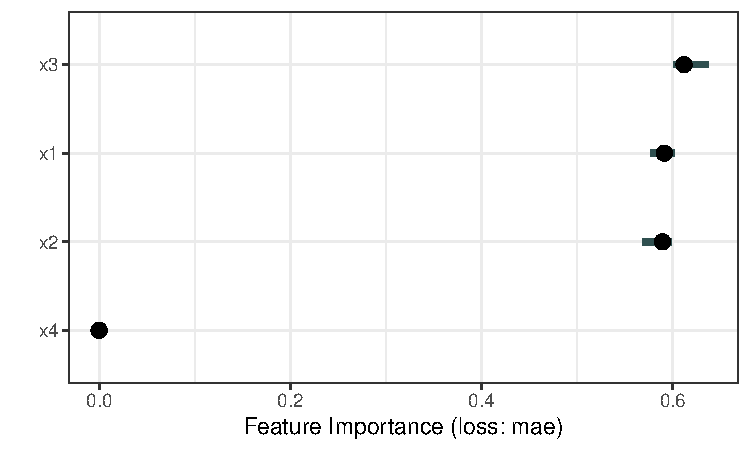
\includegraphics[width=\linewidth]{figure_man/pfi_interactions.pdf}
\end{column}
\end{columns}
\lz
\textbf{Reason:} PFI assesses importance given that all remaining features are preserved. If we first permute $x_1$ and then $x_2$, permutation of $x_2$ would have no effect on the performance (and vice versa).
\end{frame}



\begin{frame}{SAGE Idea \furtherreading{COVERT2020}
}

\textbf{SAGE:} %Leverage game-theoretic 
Use Shapley values to compute a fair attribution of importance (via model performance)\\
\lz

\textbf{Idea:} 
\begin{itemize}
    \item Feature importance attribution can be regarded as cooperative game \\
    $\leadsto$ features jointly contribute to achieve a certain model performance
    \item Players: features
    \item Payoff to be fairly distributed: model performance
    \item Surplus contribution of a feature depends on the coalition of features that are already accessible by the model
\end{itemize}
%, where each feature is a player and model performance is the payoff. The surplus contribution of a feature depends on the coalition of features that are already in the room.\\
%\pause
\lz

\textbf{Note:} 
\begin{itemize}
    \item Similar idea (called SFIMP) was proposed in \furtherreading{CASALICCHIO2018}
    \item Definition based on model refits was proposed in context of feature selection in \furtherreading{COHEN2007}
\end{itemize}

%$\Rightarrow$ Global feature importance technique\\
%$\Rightarrow$ Compute approximate Shapley values $\phi_j$ using appropriate value function 
%\lz
%$\Rightarrow$ SAGE translates SHAP into a global feature importance technique\\
%\lz
%In order to compute SAGE, approximate Shapley values $\phi_j$ as for SHAP, replacing SHAP value functions with SAGE value functions.\\
\lz

%\footnote[frame]{\fullcite{NEURIPS2020_c7bf0b7c}}
  
\end{frame}


% SAGE IDEA
\begin{frame}{SAGE - Value function}
  
 \textbf{Removal Idea:} %To deprive the model of the non-coalition features $-S$, 
 To deprive information of the non-coalition features $-S$ from the model, marginalize the prediction function over feats $-S$ to be ``dropped''.

$$\fh_S(x_S) = \E[\fh(x) | X_S = x_S]$$

%\lz

%\footnote[frame]{\fullcite{NEURIPS2020_c7bf0b7c}}

%For SAGE, value functions quantify the predictive power of a coalition $S$ in terms of reduction in risk over the mean prediction.\\
\pause
\lz

\textbf{SAGE value function:}  $$v_{\fh}(S) = \risk(\fh_{\emptyset}) - \risk(\fh_{S}), \text{ where } \risk(\fh_{S}) = \E_{Y, X_S}[L(y, \fh_S(x_S))]$$
$\leadsto$ Quantify the predictive power of a coalition $S$ in terms of reduction in risk \\
$\leadsto$ Risk of predictor $\fh_S(x_S)$ is compared to the risk of the mean prediction $\fh_{\emptyset}$


\pause
\lz

\textbf{Surplus contribution of feature $x_j$ over coalition $x_S$:}  
$$v_{\fh}(S \cup \{j\}) - v_{\fh}(S) = \risk(\fh_{S})-\risk(\fh_{S \cup \{j\}})$$
$\leadsto$ Quantifies the added value of feature $j$ when it is added to coalition $S$


\end{frame}

\begin{frame}{SAGE - marginal and cond. sampling}

When computing the marginalized prediction $\fh_S(x_S)$, the ``dropped'' features can be sampled from \\
\begin{itemize}
\item the marginal distribution $\P(x_{-S})$ $\Rightarrow$ marginal SAGE
\item the conditional distribution $\P(x_{-S}|x_S)$ $\Rightarrow$ conditional SAGE
\end{itemize}

%\lz\pause

%Interpretation of SAGE value functions differs, depending on whether conditional or marginal sampling is used.

\lz\pause

\textbf{Interpretation marginal sampling:} $v(S)$ quantifies the reliance of the model on features $x_S$
\begin{itemize}
  \item %features $x_S$ not being causal for the prediction is a sufficient condition for $v(S) = 0$
  features $x_S$ not being causal for the prediction $\Rightarrow$ $v(S) = 0$
\end{itemize}

\lz\pause

\textbf{Interpretation conditional sampling}: $v(S)$ quantifies whether variables $x_S$ contain prediction-relevant information (e.g. $y \not \indep x_S$) that is (directly or indirectly) exploited by the model
\begin{itemize}
  \item %features $x_S$ not being causal for the prediction is not a sufficient condition for $v(S) = 0$
  features $x_S$ not being causal for the prediction $\not \Rightarrow$ $v(S) = 0$
  \begin{itemize}
      \item e.g., if $x_1$ and $x_2$ are perfectly correlated, even if only $x_1$ has a nonzero coefficient, both are considered equally important
      % (see omitted variable bias as in M-plots)
  \end{itemize}
  \item under model optimality, links to mutual information or the conditional variance exist
\end{itemize}

\end{frame}


\begin{frame}{SAGE - marginal and cond. sampling}

\textbf{Example:}
%$x_1 = \epsilon_1$, $x_2 = x_1 + \epsilon_2$, $x_3 = x_2 + \epsilon_3$, $y = x_3 + \epsilon_y$ with $\epsilon_j$ independent noise terms (causal DAG: $x_1 \rightarrow x_2 \rightarrow x_3 \rightarrow y$). Assume fitting LM yields $\fh \approx 0.95 x_3 + 0.05 x_2$. 
%
\begin{columns}[T, totalwidth=\textwidth]
\begin{column}{0.4\textwidth}
\begin{itemize}
    \item $y = x_3 + \epsilon_y$\\ $x_1 = \epsilon_1$\\ $x_2 = x_1 + \epsilon_2$\\ $x_3 = x_2 + \epsilon_3$ (all $\epsilon_j$ i.i.d.)
    \item Causal DAG: $x_1 \rightarrow x_2 \rightarrow x_3 \rightarrow y$
    \item Fitted LM: $\fh \approx 0.95 x_3 + 0.05 x_2$
\end{itemize}
\end{column}
\pause
\begin{column}{0.6\textwidth}
\centerline{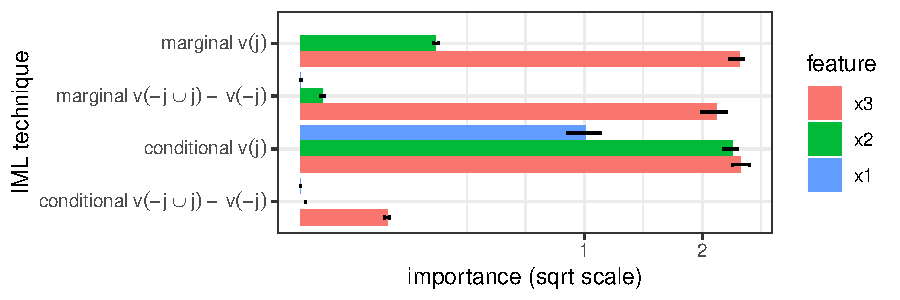
\includegraphics[width=\linewidth]{figure_man/sage_variants}}
\end{column}
\end{columns}
\lz
\begin{itemize}
    \item Marginal $v(j)$ are only nonzero for features that are used by $\fh$
    \item Conditional $v(j)$ are also nonzero for features that are not used by $\fh$ (e.g., due to correlation)
    \item For conditional value function $v$, the difference $v(-j \cup j) - v(-j)$ quantifies the unique contribution of $x_j$ over remaining features $x_{-j}$\\
    $\Rightarrow$ Since $y \indep x_1, x_2 | x_3$, only $v(\{1,2,3\}) - v(\{1, 2\})$ is nonzero (i.e., for feature $j = 3$)
\end{itemize}

\end{frame}


\begin{frame}{SAGE value functions vs. SAGE values}

\textbf{SAGE value function $v(S)$}: measure contribution of a specific feature set over the empty coalition

\lz\pause

\textbf{SAGE values $\phi_j$}: fair attribution of importance
\begin{itemize}
    \item can be computed by averaging the contribution of $x_j$ over all feat orderings
    %\item for feature permutation $\pi$ and the corresponding feature ordering $(x_{\pi(1)}, \dots, x_{phi(d)})$, for feature $x_j$ the coalition $S(j; \pi)$ is defined as the set of features preceding $x_j$, i.e. $S(j; \pi) := \{i : \pi(i) < \pi(j)\}$
    %\item the contribution of $j$ in an ordering $\pi$ is given as $v(j \cup S(j; \pi)) - v(S(j; \pi))$
    \item for feature permutation $\tau$, the contribution of $j$ in the set $\Stau$ is given as $v(\Stauj) - v(\Stau)$\\
    Note: $\Stau$ is the set of features preceding $j$ in permutation $\tau$
\end{itemize}

\lz\pause

\textbf{SAGE value approximation:} Average over the contributions for $M$ randomly sampled permutations

\begin{align*}
    \phi_j = \frac{1}{M} \sum_{m=1}^M v(\Stauj) - v(\Stau)
\end{align*}
    
\end{frame}

\begin{frame}{Interaction Example Revisited}

\textbf{Recap:} Data: $x_1, \dots, x_4$ uniformly sampled from $\{-1, 1\}$ and $y:= x_1 x_2 + x_3 + \epsilon_Y$ with $\epsilon_Y \sim N(0, 1)$. Model: $\fh(x) \approx x_1 x_2 + x_3$.\\
%
\begin{figure}
  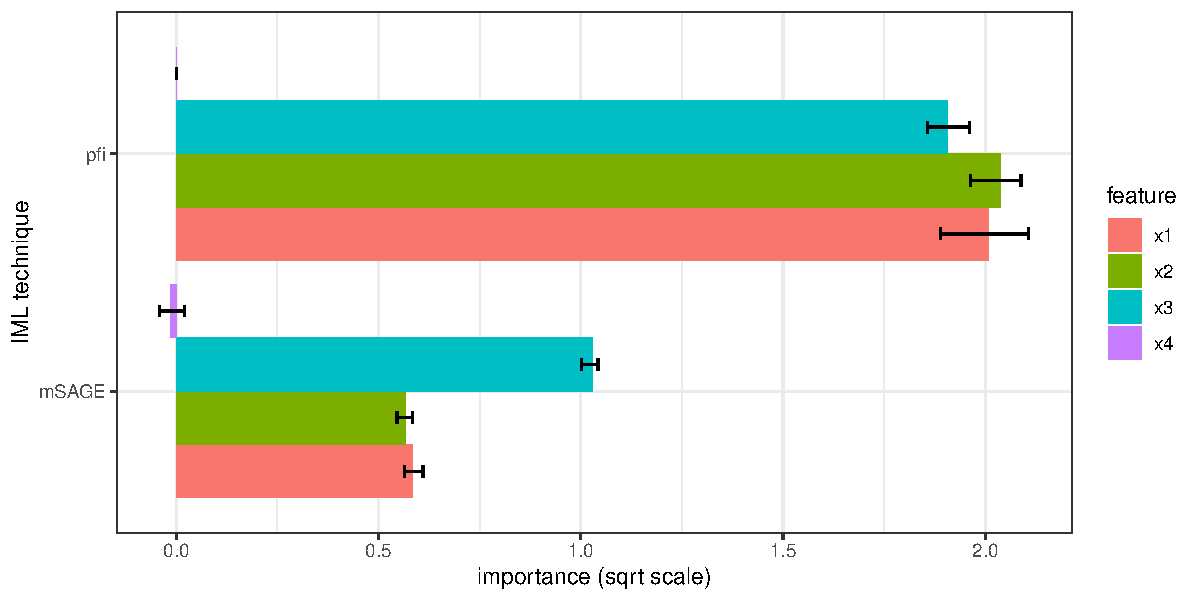
\includegraphics[width=0.65\linewidth]{figure_man/sage_pfi_interactions}
\end{figure}
%
\begin{itemize}
    \item PFI regards $x_1, x_2$ to be equally important as $x_3$
    \item Marginal SAGE fairly divides the contribution of the interaction $x_1$ and $x_2$
\end{itemize}

\end{frame}


\begin{frame}{SAGE Loss functions}

When the loss-optimal model $f^*$ is inspected using \textit{conditional-sampling} based SAGE value functions, interesting links exist.

\lz\pause
\textbf{For cross-entropy loss:} 
  \begin{itemize}
      \item value function is the mutual information:  $v_{f^*}(S) = I(y;x_S)$
      \item surplus contribution of a feature $x_j$ is the conditional mutual information: $v_{f^*}(S \cup \{j\}) - v_{f^*}(S) = I(y,x_i|x_S)$
  \end{itemize}

\lz\pause

\textbf{For MSE loss:} 
    \begin{itemize}
    \item value function is the expected reduction in variance given knowledge of the features $x_S$: $v_{f^*}(S) = Var(y) - \E[Var(y|x_S)]$
    \item surplus contribution is the respective reduction over $x_S$:
    $v_{f^*}(S \cup \{j\}) - v_{f^*}(S) = \E[Var(y|x_S)] - \E[Var(y|x_{S \cup {j}})]$
    \end{itemize}
    
\end{frame}


\begin{frame}{Implications marginal SAGE values}

Can we gain insight into whether the ...

\begin{enumerate}
    \item<1> feature $x_j$ is causal for the prediction?    \begin{itemize}
      \item for all coalitions $S$, $v(j \cup S) - v(S)$ can only be nonzero if $x_j \rightarrow \fh(x)$ (as for PFI)\\
      $\leadsto$ $\phi_j$ is only nonzero if $x_j$ is causal for the prediction
      \item $v(j \cup S) - v(S)$ may be zero due to indep. $x_j \indep y | x_S$ (as for PFI)\\
      $\leadsto$ $\phi_j$ may be zero although the feature is causal for the prediction
    \end{itemize}
    \item<2> feature $x_j$ contains prediction-relevant information about $y$?
    \begin{itemize}
      \item value functions may be nonzero despite independence due to extrapolation (as for PFI)\\
      $\leadsto$ $\phi_j$ may be nonzero without $x_j$ being dependent with $y$
      \item value functions may be zero despite $x_j$ containing prediction-relevant information due to underfitting (as for PFI)\\
      $\leadsto$ $\phi_j$ may be zero although prediction-relevant information contained
    \end{itemize}
    \item<3> model requires access to $x_j$ to achieve its prediction performance?    
    \begin{itemize}
      \item like PFI, in general marginal value functions do not allow insight into unique contribution $\leadsto$ no insight from $\phi_j$
    \end{itemize}
\end{enumerate}

\end{frame}
%
\begin{frame}{Implications conditional SAGE values}

Can we gain insight into whether the ...

\begin{enumerate}
    \item<1> feature $\xj$ is causal for the prediction?
    \begin{itemize}
      \item value funcs may be nonzero although feature is not directly used by $\fh$\\
      $\leadsto$ nonzero $\phi_j$ does not imply $\xj \rightarrow \hat{y}$
      \item value functions may be zero although feature may be used by the model, e.g. if feature is independent with $y$ and all other features \\ $\leadsto$ zero $\phi_j$ does not imply $\xj \not \rightarrow \hat{y}$
    \end{itemize}
    \item<2> feature $\xj$ contains prediction-relevant information about $y$?
    \begin{itemize}
      \item e.g. for cross-entropy optimal $\fh$, $v(j)$ measures mutual info. $I(y;x_j)$
      $\leadsto$ prediction-relevance implies nonzero $\phi_j$
      \item $x_j \indep y$ does not imply $x_j \indep y | x_S$ and consequently does not imply $v(j \cup S) - v(S) = 0$
      $\leadsto$ $\phi_j$ may be nonzero although $\xj \indep y$
    %   \item $x_j \indep y$ in general does not imply $x_j \indep y | x_S$ and consequently does not imply that $v(j \cup S) - v(S) = 0$\\
    %   $\leadsto$ $\phi_j$ may be nonzero although $\xj \indep y$
    \end{itemize}
    \item<3> model requires access to $x_j$ to achieve its prediction performance?  
    \begin{itemize}
        \item e.g. for cross-entropy optimal $\fh$, surplus contrib. $v(j \cup -j) - v(-j)$ captures the conditional mutual information $I(y;x_j|x_{-j})$\\
        $\leadsto$ $\phi_j$ is nonzero for features with unique contribution
        \item $x_j \indep y | x_{-j}$ does not imply $x_j \indep y | x_S$ (cond. w.r.t. to arbitrary coalitions $S$)\\
        $\leadsto$ $\phi_j$ may be nonzero although feature has no unique contrib.
    \end{itemize}
\end{enumerate}

\end{frame}

% \begin{frame}
%   \printbibliography
% \end{frame}

\begin{frame}{Deep dive: Shapley axioms for SAGE}

The Shapley axioms can be translated into properties of SAGE. The interpretation depends on whether conditional or marginal sampling is used.
%
\begin{table}
  \centering
  \begin{tabular}{l | l }
  Shapley property $\implies$ & conditional SAGE property \\
  \hline
  efficiency & $\sum_{i=1}^p \phi_j(v) = \risk(\fh_\emptyset) - \risk(\fh)$\\ % \hline
  symmetry & $x_j = x_i \implies \phi_i = \phi_j$ \\ 
  linearity & $\phi_j$ expectation of per-instance\\
  & conditional SHAP applied to model loss\\ %\hline
  monotonicity & given models $f, f'$, if  $\forall S:$\\
  &$v_f(S \cup j) - v_f(S) \geq v_{f'}(S \cup j) - v_{f'}(S)$ \\
  &then $\phi_j(v_f) \geq \phi_j(v_{f'})$\\ %\hline
  dummy & if $\forall S: \fh(x) \indep x_j | x_S \Rightarrow \phi_j = 0$
  \end{tabular}
\end{table}

\end{frame}

\begin{frame}{Deep dive: Shapley axioms for SAGE}
%
The Shapley axioms can be translated into properties of SAGE. The interpretation depends on whether conditional or marginal sampling is used.
%
\begin{table}
  \centering
  \begin{tabular}{l | l }
  Shapley property $\implies$ & marginal SAGE property \\
  \hline
  efficiency & $\sum_{i=1}^p \phi_j(v) = \risk(\fh_\emptyset) - \risk(\fh)$\\
  symmetry & no intelligible implication \\
  linearity & $\phi_j$ expecation of per-instance\\
  & marginal SHAP applied to model loss\\
  monotonicity & given models $f, f'$, if  $\forall S:$\\
  &$v_f(S \cup j) - v_f(S) \geq v_{f'}(S \cup j) - v_{f'}(S)$ \\
  &then $\phi_j(v_f) \geq \phi_j(v_{f'})$\\
  dummy & model invariant to $x_j \Rightarrow \phi_j = 0$\\
  \end{tabular}
\end{table}
%
\end{frame}

\endlecture
\end{document}
